%!TEX TS-program = xelatex
%!TEX encoding = UTF-8 Unicode

\documentclass[11pt,tikz,border=1]{standalone}
\usetikzlibrary{positioning}

\begin{document}
  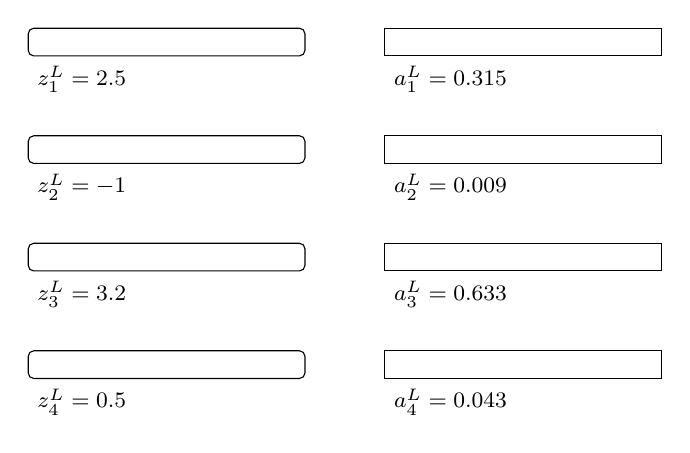
\begin{tikzpicture}[
    font=\footnotesize,
    base/.style={rectangle,draw,minimum width=100pt,minimum height=10pt},
    slidebar/.style={base,rounded corners=2pt},
    colorbar/.style={base}
  ]

  \node(s1) [slidebar] {};
  \node(z1) [below,anchor=north west] at (s1.south west) {$z^L_1 = 2.5$};

  \node(b1) [colorbar,right=of s1] {};
  \node(a1) [below,anchor=north west] at (b1.south west) {$a^L_1 = 0.315$};

  \node(s2) [slidebar,below=of s1] {};
  \node(z2) [below,anchor=north west] at (s2.south west) {$z^L_2 = -1$};

  \node(b2) [colorbar,right=of s2] {};
  \node(a2) [below,anchor=north west] at (b2.south west) {$a^L_2 = 0.009$};

  \node(s3) [slidebar,below=of s2] {};
  \node(z3) [below,anchor=north west] at (s3.south west) {$z^L_3 = 3.2$};

  \node(b3) [colorbar,right=of s3] {};
  \node(a3) [below,anchor=north west] at (b3.south west) {$a^L_3 = 0.633$};

  \node(s4) [slidebar,below=of s3] {};
  \node(z4) [below,anchor=north west] at (s4.south west) {$z^L_4 = 0.5$};

  \node(b4) [colorbar,right=of s4] {};
  \node(a4) [below,anchor=north west] at (b4.south west) {$a^L_4 = 0.043$};

  \end{tikzpicture}
\end{document}
